\documentclass{beamer}

\mode<presentation> {

\usetheme{Madrid}
}

\usepackage{graphicx}
\usepackage{booktabs}
\usepackage[T2A]{fontenc}
\usepackage[utf8]{inputenc}
\usepackage[russian, english]{babel}
\usepackage{enumerate}
\usepackage{setspace}
\usepackage{listing}

\newenvironment{MyList}[1][4pt]{
	\begin{enumerate}[1.]
		\setlength{\parskip}{0pt}
		\setlength{\itemsep}{#1}
	}{       
\end{enumerate}
}
\newenvironment{InnerMyList}[1][0pt]{
	\vspace*{-0.5em}
	\begin{enumerate}[a)]
		\setlength{\parskip}{#1}
		\setlength{\itemsep}{0pt}
	}{
\end{enumerate}
}

%----------------------------------------------------------------------------------------
%	TITLE PAGE
%----------------------------------------------------------------------------------------

\title[Позиционирование видеокамеры]{Определение положения и ориентации видеокамеры}

\author[Григорий Бартош]{
	Григорий Бартош\\
	\scriptsize Руководитель: Александр Смирнов, компания Геоскан
}
\institute[СПб АУ]{Санкт-Петербургский Академический Университет}
\date[30.05.2018]{Среда, 30 мая 2018 года}

\begin{document}

\begin{frame}
\titlepage
\end{frame}

\begin{frame}
\frametitle{Overview}
\tableofcontents
\end{frame}

%----------------------------------------------------------------------------------------
%	PRESENTATION SLIDES
%----------------------------------------------------------------------------------------

%------------------------------------------------
\section{Постановка задачи}
%------------------------------------------------

\begin{frame}
\frametitle{Постановка задачи}
\textbf{Дано}
\begin{enumerate}
	\item 
	Модель камеры\\
	\begin{InnerMyList}
		\item
		Разрешение камеры: $Width \times Height$
		
		\item
		Угловой размер: $\alpha_{Height}$
	\end{InnerMyList}
	
	\item
	Множество из $n$ точек\\
	\begin{InnerMyList}
		\item
		Координаты в трехмерном пространстве:
			$X = \begin{pmatrix} 
			x \\
			y \\
			z
			\end{pmatrix}$
		
		\item
		Координаты на изображение: 
			$P_{pix} = \begin{pmatrix} 
			u_{pix} \\
			v_{pix}
			\end{pmatrix}$
	\end{InnerMyList}
\end{enumerate}

\textbf{Задача.}\\
\text{По данной информации требуется найти}
\begin{enumerate}
	\item 
	Координаты камеры:
		$t = \begin{pmatrix} 
		t_x \\
		t_y \\
		t_z
		\end{pmatrix}$
	
	\item
	Эйлеровы углы поворота: $\omega_x, \omega_y, \omega_z$
\end{enumerate}
\end{frame}

%------------------------------------------------

\begin{frame}
	\frametitle{Так а что надо?}
	\textbf{Введем функцию ошибки, которую будем минимизировать.}
	
	\begin{columns}[c]
		\column{.35\textwidth}
		$T = \left(\begin{array}{@{}c|c@{}}
		R & t
		\end{array}\right)$
		
		\column{.65\textwidth}
		$R$ --- трехмерная матрица поворота\\
		$T$ --- матрица трансформации
	\end{columns}
	
	\begin{columns}[c]
		\column{.35\textwidth}
		$P_H := \begin{pmatrix} 
		u \\
		v \\
		1
		\end{pmatrix}$
		
		\column{.65\textwidth}
		$P_H$ --- луч задаваемый точкой на изображение
	\end{columns}
	
	\begin{columns}[c]
		\column{.35\textwidth}
		$P := \begin{pmatrix} 
		0 & -1 & v \\
		1 & 0 & -u \\
		-v & u & 0
		\end{pmatrix}$
		
		\column{.65\textwidth}
		$P$ --- кососимметричная матрица $P_H$
	\end{columns}
	
	Тогда для идеального случая будет верно: 
	$$ P T 
	\begin{pmatrix} 
	X \\\hline
	1
	\end{pmatrix} = \vec{0} $$
	
	Ошибкой будет сумма отклонений, и она должна стремится к нулю.
	$$ (P T 
	\begin{pmatrix} 
	X \\\hline
	1
	\end{pmatrix})
	\cdot
	(P T 
	\begin{pmatrix} 
	X \\\hline
	1
	\end{pmatrix}) \rightarrow \min$$
\end{frame}

%------------------------------------------------
\section{Обзор существующих решений}
%------------------------------------------------

\begin{frame}
\frametitle{Обзор существующих решений}
	\begin{itemize}	
	\item{\bf Алгоритмы, работающие за время $\omega(n)$ }\\
	О них чуть позже.\\
	\textbf{Минусы:} Нелинейное время работы.
		
	\item{\bf Bundle adjustment}\\
	Широко используется при решение задачи 3D SLAM. Примеры:\\
	\begin{InnerMyList}
		\item
		PTAM (2007 год)
		
		\item
		ORB-SLAM (2015 год)
	\end{InnerMyList}
	 Более общая задача.\\
	 \textbf{Минусы:} Нелинейное время работы.

	\item{\bf Поиск минимумы ошибки стандартными средствами}
	Пример:\\
	Метод отжига. Автор: Андрей Крутиков (СПбАУ, 2015 год)\\
	\textbf{Минусы:} Большая константа + неточный.
\end{itemize}
\end{frame}

%------------------------------------------------
\section{Решение}
\subsection{Трансформации при малых углах}
%------------------------------------------------

\begin{frame}
\frametitle{Идея I: Трансформации при малых углах}
	Матрица поворота строится из поворотов вокруг осей.
	$$R = 
	\begin{pmatrix} 
	\cos{\omega_z} & -\sin{\omega_z} & 0 \\
	\sin{\omega_z} & \cos{\omega_z} & 0 \\
	0 & 0 & 1
	\end{pmatrix}
	\begin{pmatrix} 
	\cos{\omega_y} & 0 & \sin{\omega_y} \\
	0 & 1 & 0 \\
	-\sin{\omega_y} & 0 & \cos{\omega_y}
	\end{pmatrix}
	\begin{pmatrix} 
	1 & 0 & 0 \\
	0 & \cos{\omega_x} & -\sin{\omega_x} \\
	0 & \sin{\omega_x} & \cos{\omega_x}
	\end{pmatrix}$$
	
	Если повороты малые (до $\approx 20^\circ$), можно линеризовать матрицу.
	$$ R = 
	\begin{pmatrix} 
	1 & -\omega_z & 0 \\
	\omega_z & 1 & 0 \\
	0 & 0 & 1
	\end{pmatrix}
	\begin{pmatrix} 
	1 & 0 & \omega_y \\
	0 & 1 & 0 \\
	-\omega_y & 0 & 1 
	\end{pmatrix}
	\begin{pmatrix} 
	1 & 0 & 0 \\
	0 & 1 & -\omega_x \\
	0 & \omega_x & 1
	\end{pmatrix}$$
	$$R = \begin{pmatrix} 
	1 & -\omega_z & \omega_y \\
	\omega_z & 1 & -\omega_x \\
	-\omega_y & \omega_x & 1
	\end{pmatrix}$$
\end{frame}

%------------------------------------------------
\subsection{Нахождение малых углов}
%------------------------------------------------

\begin{frame}
	\frametitle{Идея II: Нахождение малых углов}
	Нужно найти $T$ так, чтобы:
	$ (P T 
	\begin{pmatrix} 
	X \\\hline
	1
	\end{pmatrix})
	\cdot
	(P T 
	\begin{pmatrix} 
	X \\\hline
	1
	\end{pmatrix}) \rightarrow \min$
	
	Посмотрим повнимательнее:
	$$T \begin{pmatrix} 
	X \\\hline
	1
	\end{pmatrix} = 
	\left(\begin{array}{@{}ccc|c@{}}
	1 & -\omega_z & \omega_y & t_x \\
	\omega_z & 1 & -\omega_x & t_y \\
	-\omega_y & \omega_x & 1 & t_z
	\end{array}\right)
	\begin{pmatrix} 
	x \\
	y \\
	z \\
	1
	\end{pmatrix} =
	\begin{pmatrix} 
	x - \omega_z y + \omega_y z + t_x \\
	y + \omega_z x - \omega_x z + t_y \\
	z - \omega_y x + \omega_x y + t_z
	\end{pmatrix} +
	\begin{pmatrix} 
	x \\
	y \\
	z
	\end{pmatrix}$$
	
	Пусть
	$G = 
	\begin{pmatrix} 
		1 & 0 & 0 &  0 &  z & -y \\
		0 & 1 & 0 & -z &  0 &  x \\
		0 & 0 & 1 &  y & -x &  0 \\
	\end{pmatrix},
	\mu = 
	\begin{pmatrix} 
		t_x \\
		t_y \\
		t_z \\
		\omega_x \\
		\omega_y \\
		\omega_z 
	\end{pmatrix}$
	
	Используя введенные переменные можем переписать равенство:
	$$T \begin{pmatrix} 
	X \\\hline
	1
	\end{pmatrix} = G \mu + X$$
\end{frame}

%------------------------------------------------

\begin{frame}
\begin{spacing}{1.5}
	\frametitle{Идея II: Нахождение малых углов}
	\begin{columns}[c]
		\column{.5\textwidth}
		$(P G \mu + P X) \cdot (P G \mu + P X) \rightarrow \min$
		
		\column{.5\textwidth}
		Перепишем функцию минимизации
	\end{columns}
	
	\begin{columns}[c]
		\column{.5\textwidth}
		$G^T P^T (P G \mu + P X) = 0$
		
		\column{.5\textwidth}
		Приравняем производную к $0$
	\end{columns}
	
	\begin{columns}[c]
		\column{.5\textwidth}
		$G^T P^T P G \mu = - G^T P^T P X$
		
		\column{.5\textwidth}
		Получили простую СЛУ
	\end{columns}
	
	\begin{columns}[c]
		\column{.5\textwidth}
		$(\sum G^T P^T P G) \mu = - \sum G^T P^T P X$
		
		\column{.5\textwidth}
		Суммируем по всем точкам
	\end{columns}
	
	Получили систему \textbf{всего из 6} уравнений и неизвестных.
	
	Найдем матрицу поворота:
	\begin{columns}[c]
		\column{.5\textwidth}
		$R = I + \frac{\sin{\theta}}{\theta} \omega_{\times} + \frac{1 - \cos{\theta}}{\theta^2} \omega_{\times}^2$
		
		\column{.5\textwidth}
		$I$ --- единичная матрица\\
		$\theta = \sqrt{\omega_x^2 + \omega_y^2 + \omega_z^2}$\\
		$\omega_{\times} = 
		\begin{pmatrix} 
		0 & -\omega_z & \omega_y \\
		\omega_z & 0 & -\omega_x \\
		-\omega_y & \omega_x & 0
		\end{pmatrix}$
	\end{columns}
\end{spacing}
\end{frame}

%------------------------------------------------
\subsection{Оценка времени работы}
%------------------------------------------------

\begin{frame}
\frametitle{И где ответ?}
	$T_{Strat}$ --- произвольная трансформация.\\
	$T_{res} = T_i T_{res}$ --- итеративно уточняем ответ.\\
	\textbf{И долго его уточнять? Нет!}\\
	%TODO распределение

\end{frame}

%------------------------------------------------

\begin{frame}
	\frametitle{А мы точно получим ответ?}
	Не совсем...
	%TODO вероятность взять хорошую
	
\end{frame}

%------------------------------------------------

\begin{frame}
	\frametitle{Однако!}
	%TODO линии 100
	
\end{frame}

%------------------------------------------------

\begin{frame}
	\frametitle{Скорость схождения}
	%TODO линии все
	
\end{frame}

%------------------------------------------------

\begin{frame}
	\frametitle{10-я итерация}
	%TODO 10я итерация
	
\end{frame}

%------------------------------------------------

\begin{frame}[fragile]
\begin{spacing}{1.5}
	\frametitle{Число итераций}
	
	$ITR_{check} = 10$
	
	$E$ --- математическое ожидание числа итераций.\\
	\begin{columns}[c]
		\column{.05\textwidth}
		$E = $
		
		\column{.95\textwidth}
		$(1-P[\text{get good}])(ITR_{check} + E) +$
	\end{columns}
	\begin{columns}[c]
		\column{.05\textwidth}
		
		\column{.95\textwidth}
		$P[\text{get good}](E[\text{itr for good}] + P[\text{out of time}](ITR_{check} + E))$
	\end{columns}
	
	$$E = \frac{(1-P[\text{get good}])ITR_{check} + P[\text{get good}]E[\text{itr for good}]}{P[\text{get good}] - P[\text{out of time}]}$$
	
	$$E \approx 36.4733$$
\end{spacing}
\end{frame}

%------------------------------------------------
\section{Итог}
%------------------------------------------------

\begin{frame}
\frametitle{Итог}
	\centerline{Получили \textbf{быстрый} и \textbf{точный} алгоритм.}
	
	\centerline{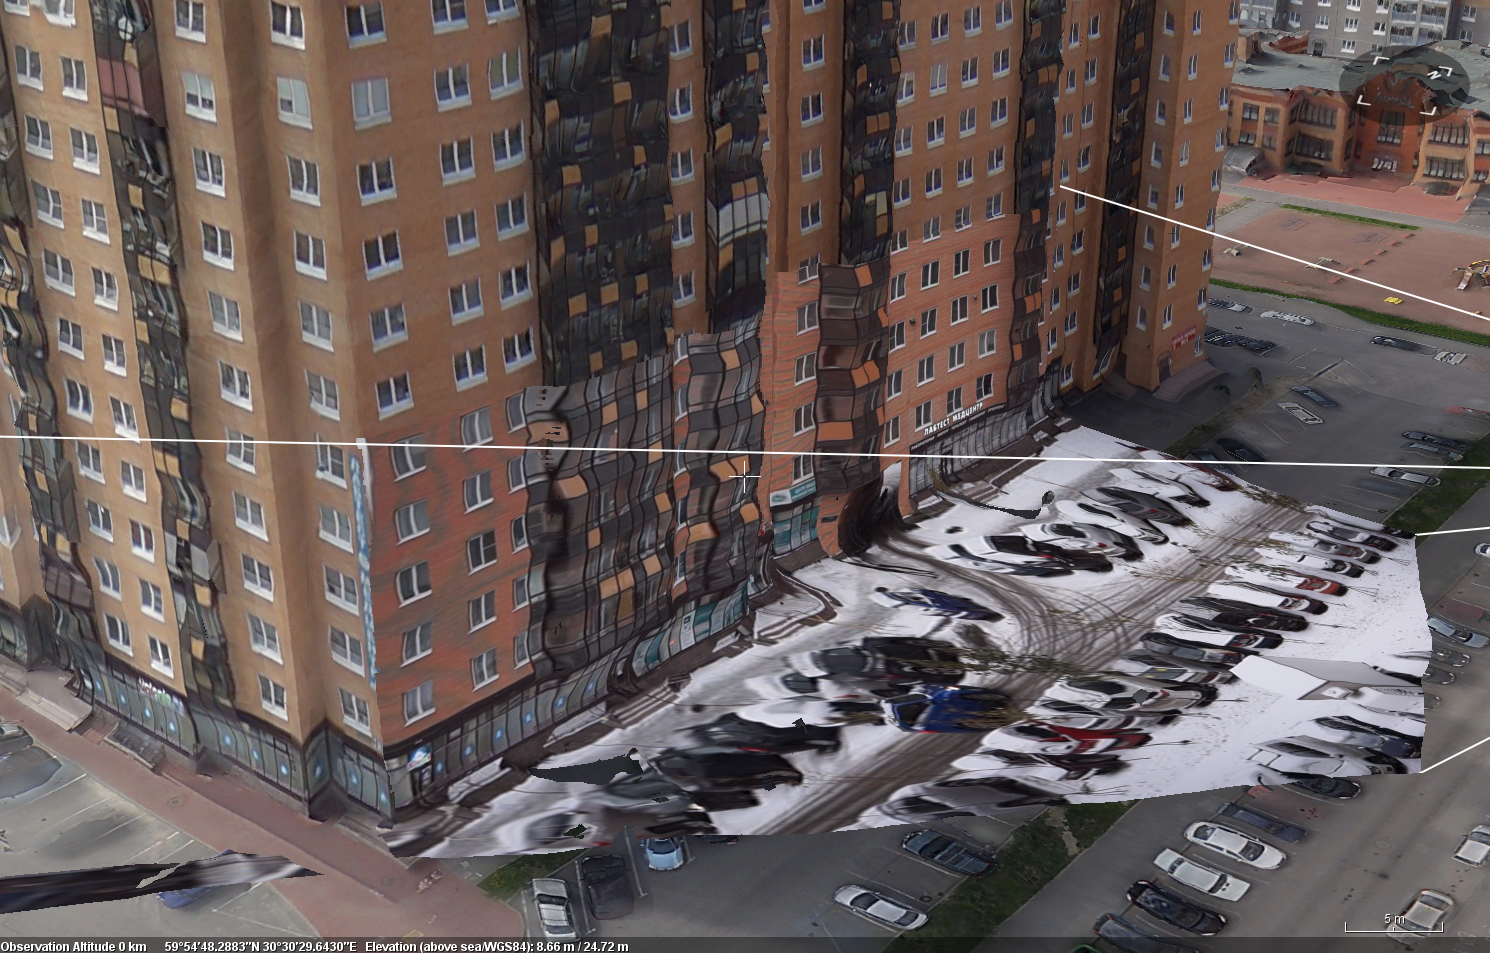
\includegraphics[scale=0.26]{sample.png}}
\end{frame}

%----------------------------------------------------------------------------------------

\end{document}